%Pakete;
%A4, Report, 12pt
\documentclass[ngerman,a4paper,12pt]{scrreprt}
\usepackage[a4paper, right=20mm, left=20mm,top=30mm, bottom=30mm, marginparsep=5mm, marginparwidth=5mm, headheight=7mm, headsep=15mm,footskip=15mm]{geometry}

%Papierausrichtungen
\usepackage{pdflscape}
\usepackage{lscape}

%Deutsche Umlaute, Schriftart, Deutsche Bezeichnungen
\usepackage[utf8]{inputenc}
\usepackage[T1]{fontenc}
\usepackage[ngerman]{babel}

%quellcode
\usepackage{listings}
\usepackage{verbatim}

%tabellen
\usepackage{tabularx}
\usepackage{csvsimple}

%listen und aufzählungen
\usepackage{paralist}

%farben
\usepackage[svgnames,table,hyperref]{xcolor}

%font
\usepackage{helvet}
\renewcommand{\familydefault}{\sfdefault}

%Abkürzungsverzeichnisse
\usepackage[printonlyused]{acronym}

%Bilder
\usepackage{graphicx} % Bilder
\usepackage{float}	  %"Floating" Objects, Bilder, Tabellen...

%Pdf einbinden
\usepackage{pdfpages}


%Dokumenteigenschaften
\title{Dkoumentation Simulationsprojekt Hardrock}
\def\author{Reto Schelbert, Simon Schreiber, Tobias Blaser, Urs Baumann}
\providecommand{\teacher}{A. Rinkel}
\providecommand{\room}{5.002}
\providecommand{\versionnumber}{1.2}
\date{\today{}, Rapperswil}


%Kopf- /Fusszeile
\usepackage{fancyhdr}
\usepackage{lastpage}

\pagestyle{fancy}
\fancyhf{} %alle Kopf- und Fußzeilenfelder bereinigen
\fancyhead[L]{System Modelling and Simulation} %Kopfzeile links
\fancyhead[C]{Projekt: Hardrock} %Kopfzeile mitte
\fancyhead[R]{Seite \thepage/\pageref{LastPage}} %Kopfzeile rechts
\renewcommand{\headrulewidth}{0.4pt} %obere Trennlinie
\fancyfoot[L]{\jobname} %Fusszeile links
\fancyfoot[C]{Version: \versionnumber} %Fusszeile mitte
\fancyfoot[R]{\today{}} %Fusszeile rechts
\renewcommand{\footrulewidth}{0.4pt} %untere Trennlinie

%Kopf-/ Fusszeile auf chapter page
\fancypagestyle{plain} {
	\fancyhf{} %alle Kopf- und Fußzeilenfelder bereinigen
	\fancyhead[L]{System Modelling and Simulation} %Kopfzeile links
	\fancyhead[C]{Projekt: Hardrock} %Kopfzeile mitte
	\fancyhead[R]{Seite \thepage/\pageref{LastPage}} %Kopfzeile rechts
	\renewcommand{\headrulewidth}{0.4pt} %obere Trennlinie
	\fancyfoot[L]{\jobname} %Fusszeile links
	\fancyfoot[C]{Version: \versionnumber} %Fusszeile mitte
	\fancyfoot[R]{\today{}} %Fusszeile rechts
	\renewcommand{\footrulewidth}{0.4pt} %untere Trennlinie
}

\usepackage{changepage}

%links, verlinktes Inhaltsverzeichnis, PDF Inhaltsverzeichnis
\usepackage[bookmarks=true,
bookmarksopen=true,
bookmarksnumbered=true,
breaklinks=true,
colorlinks=true,
linkcolor=black,
anchorcolor=black,
citecolor=black,
filecolor=black,
menucolor=black,
pagecolor=black,
urlcolor=black
]{hyperref} % Paket muss unbedingt als letzes eingebunden werden!

\begin{document}

%Titel und Inhaltsverzeichnis
\thispagestyle{empty}
\begin{titlepage}
	\begin{center}

	\vspace*{40mm}
	
	\begin{figure}[htp]
		\centering
		
\includegraphics[width=0.60\textwidth]{img/Hard-Rock-Cafe-Logo-Black-White.png}
	\end{figure}		
	\vspace*{20mm}
	
	{\fontsize{40}{48} \selectfont Projekt Hardrock \\[10mm]}
	{\fontsize{32}{48} \selectfont Dokumentation \\[5mm]}	
	\vspace*{20mm}
	\author

\end{center}
\end{titlepage}
\clearpage

\chapter*{Änderungsnachweis}
\begin{tabularx}{\textwidth}{|cXlr|} % Versionstabelle, Rahmen links und rechts
		\hline
		\textbf{Version} & \textbf{Änderung} & \textbf{Autor} & \textbf{Datum}\\
		\hline
		1.0 & Dokumentenentwurf & Tobias Blaser & 24.03.2013 \\
		1.1 & Entwurf Konzept & Tobias Blaser & 28.03.2013 \\
		1.2 & Ergänzungen und Korrekturen & Reto Schelbert & 03.04.2013 \\
		1.3 & Überarbeitung Konzept (Word Model) & Tobias Blaser & 08.04.2013 \\
		1.4 & Modell \& Verteilungsfunktionen & Tobias Blaser & 03.05.2013 \\
		1.5 & Simulation & Alle & 10.05.2013 \\
		1.6 & Modellbeschreibungen & Tobias Blaser & 11.05.2013\\
		1.7 & Plausibilitätscheck, Szenarios & Alle & 13.05.2013\\
		1.8 & Szenarien, Auswertung & Urs Baumann, Tobias Blaser & 17.05.2013\\
		1.9 & Auswertung, Überarbeitungen & Alle & 24.05.2013\\
		\hline
\end{tabularx}

% Inhaltsverzeichnis
\tableofcontents


\chapter{Konzept}


\section{Model}
Als Ausgangskonzept wird das Hardrock in Atlantic City verwendet.
\begin{figure}[htp]
	\centering
		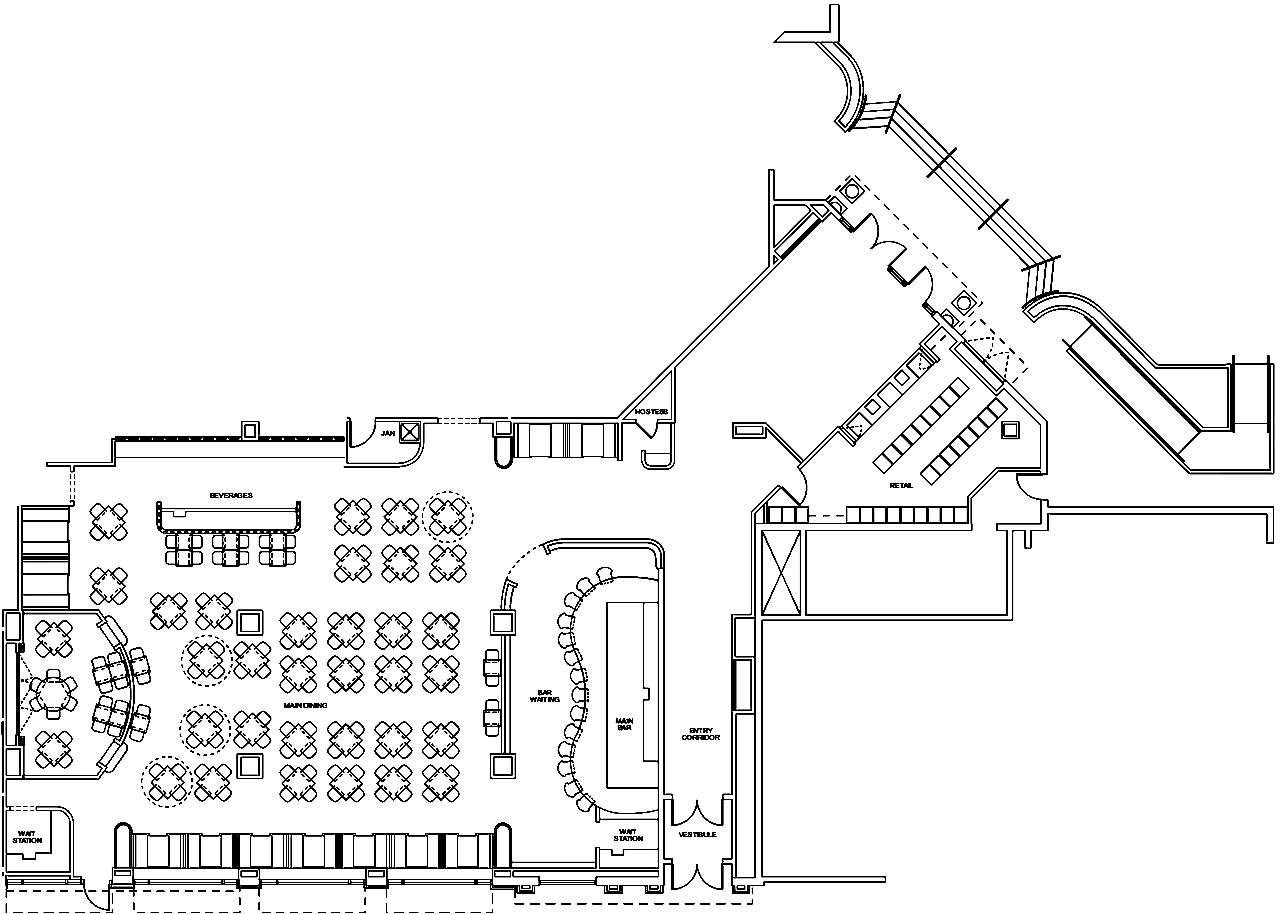
\includegraphics[width=1\textwidth]{img/hardrock-plan.png}
		\caption[Gebäudeplan Hardrock]{Gebäudeplan Hardrock Cafe, Atlantic City (Quelle: www.hardrock.com, 25.03.13)}
		\label{planHardrock}
\end{figure}

\subsection{Eingangsbereich}
Vor dem Eingangsbereich warten die Gäste in einer Schlange, bis an der Bar Plätze frei werden. Ziel ist, diese Warteschlange so kurz wie möglich zu halten. Die Gäste sollen stattdessen an der Bar warten und zum Konsumieren angeregt werden.

Ist die Schlange vor dem Eingang zu lang, gehen Gäste wieder ohne Besuch im Restaurant. Dies soll möglichst vermieden werden, da diese Gäste keinen Umsatz bescheren.

\subsection{Bar}
Die Bar dient als Warteschlange für die Gäste, bis Plätze an einem Tisch frei werden. Gäste werden an der Bar bedient und konsumieren Getränke.
Das Servierpersonal an der Bar soll in unserer Simulation nicht berücksichtigt werden. Grund dafür ist die Unabhängigkeit des Barbereichs vom Rest des Lokals. Das heisst: Das Barpersonal ist nicht in der Lage, kurzzeitig die Bar zu verlassen und Tische zu bedienen. Weil es nur für die Ausgabe der Getränke verantwortlich ist, kann es in der Simulation vernachlässigt werden, ohne das System zu verfälschen.

???
Ziel ist es, dass an der Bar möglichst viele Plätze besetzt sind, weil dies Einnahmen durch Konsumation generiert. Gleichzeitig sollte vor der Türe die Schlange möglichst klein sein oder gar nicht existieren, damit keine Gäste an der Kälte warten müssen, oder sogar wieder gehen. Die Wartezeit an der Bar sollte nicht mehr als ein bis zwei Drinks betragen, damit niemand wieder geht, bevor ein Tisch frei wird.

$\rightarrow$ Annahme Dauer eines Drinks an der Bar: ca. eine Viertelstunde bis 20 Minuten.

\subsection{Tische}
Am Tisch werden ein bis drei Gänge gegessen. In einem ersten Schritt soll dies sehr einfach abgebildet werden. Auf eine komplexe Menüsimulation in der Granularität der einzelnen Gänge wird verzichtet.

Das Servierpersonal kommt einmal und nimmt Bestelllungen auf. Das Servierpersonal ist somit für eine bestimmte Zeit belegt und anschliessend wieder frei. 

Das Szenario Teller und Karte bringen soll erst in einem zweiten Schritt modelliert werden, je nach verfügbarer Projektzeit.

In der realen Welt bestehen die Tische aus Vierertischen. Ankommende Gruppen müssen aufgeteilt oder Tische zusammengeschoben werden. Bei weniger als 4 Personen kann es zu leeren Plätzen kommen. Um die Simulation nicht unnötig aufzublähen, soll dies nicht berücksichtigt werden in der Simulation.
Die Anzahl Plätze werden fix gewählt anhand des Beispiels von Atlantic City (250 Plätze).

Nach dem Esssen  verlassen die Gäste das Hardrock und der Tisch wird frei für neue Gäste.
In der Realität kann es durchaus vorkommen, dass Gäste nochmals an die Bar zurückkehren.


\subsection{Küche}
	In der Küche werden die verschiedenen Mahlzeiten gekocht und angerichtet. Die Köche arbeiten gleichzeitig an mehreren Menüs und versuchen, zusammengehörende Menüs möglichst gleichzeitig fertigzustellen.

	In einem ersten Schritt soll die Küche sehr rudimentär simuliert werden. Es existieren Köche, die eine bestimmte Zeit benötigen, um Essen zuzubereiten. Paralleles Kochen von Menüs soll nur durch entsprechende Verkürzung der Gesammtkochzeit abgebildet werden.

	In einem Zweiten Schritte könnnten verschiedene Köche, die pro Essen und Gang an eine bestimmte Zeit gebunden sind, modelliert werden.


\section{Bewegungsabläufe}
	\begin{figure}[H]
		\centering
			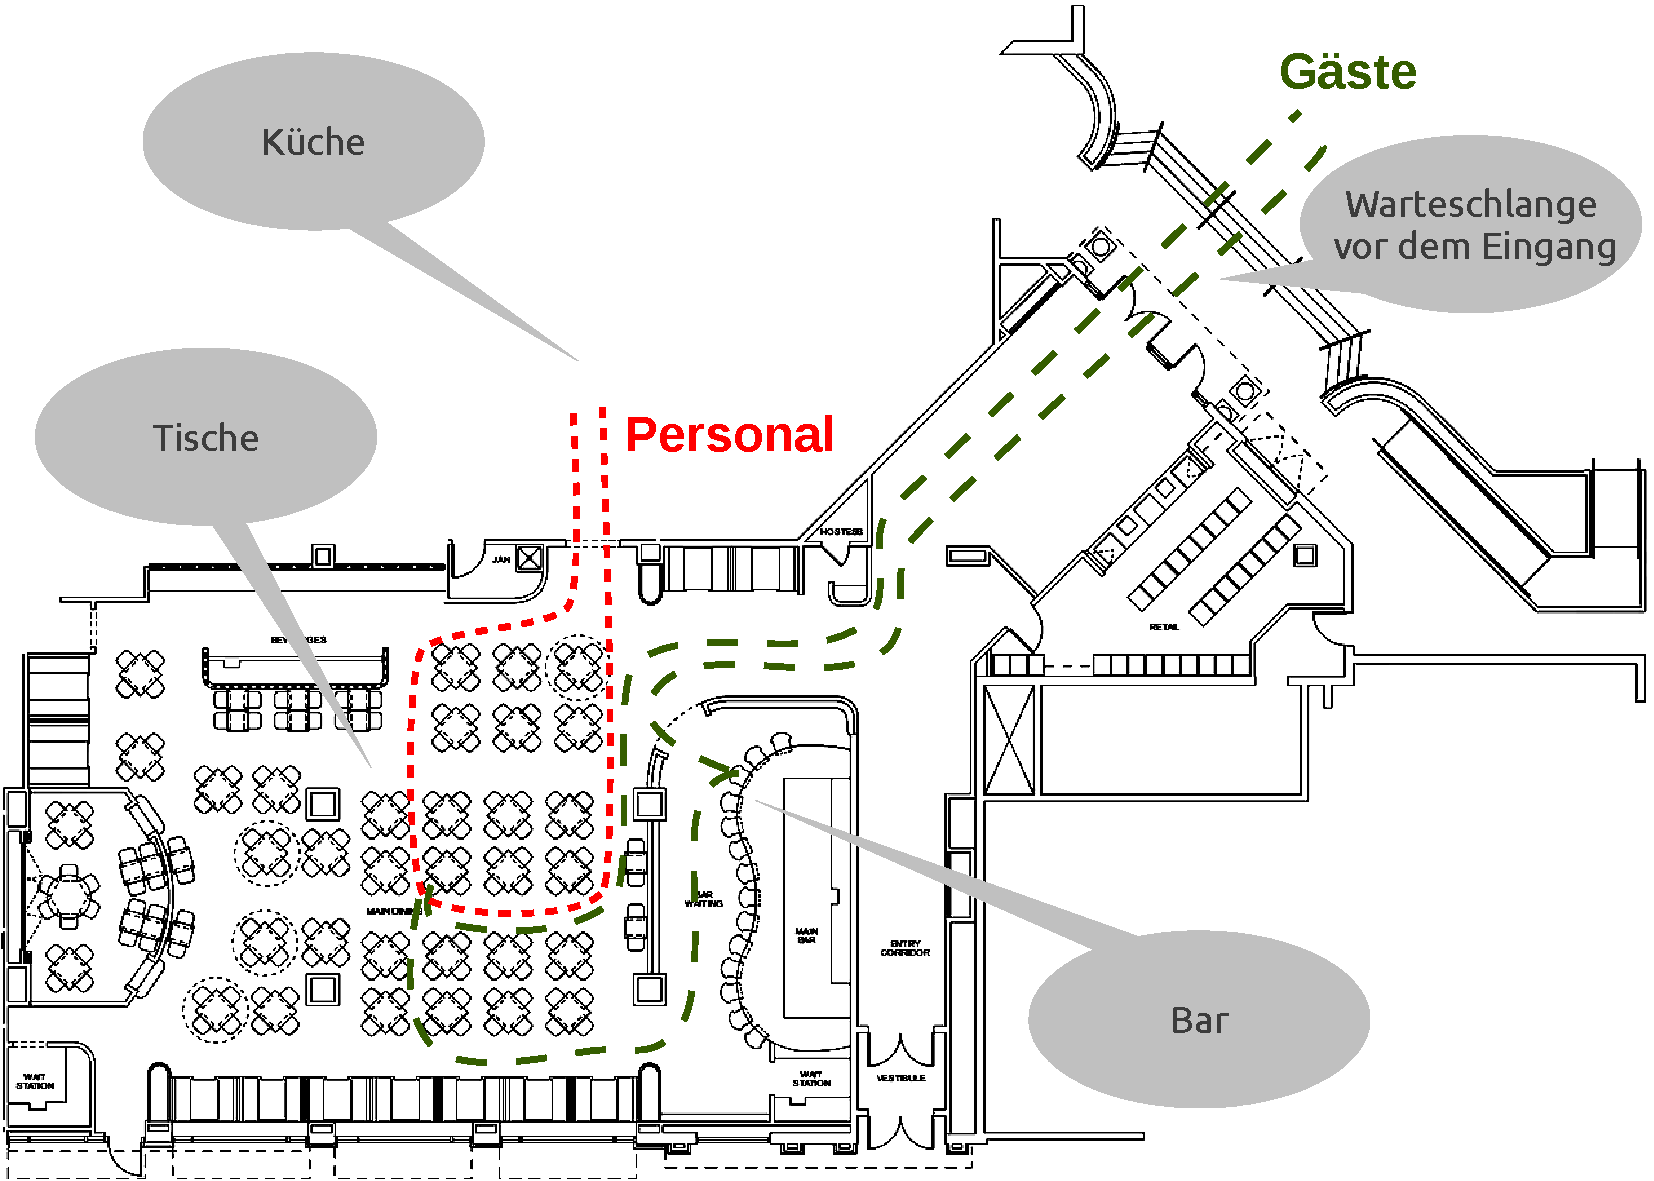
\includegraphics[width=1\textwidth]{img/hardrockSchema.pdf}
			\caption[Bewegungsschema Hardrock]{Bewegungsschema im Hardrock Cafe, Atlantic City (Beispiel Bewegungsablauf an einem Tisch)}
			\label{schemaHardrock}
	\end{figure}

	Die Verschiedenen Aktivitäten finden an unterschiedlichen Orten im Café statt. Die daraus resultierenden Wegzeiten variieren stark, unterliegen sehr komplexen Verteilungen und können nur empirisch ermittelt werden.

	\subsection{Gäste}
		\begin{itemize}
			\item Gäste benötigen eine variierende Zeit um vom Eingang an die Bar zu gelangen, ??? wobei das Laufverhalten auch von der Gruppengrösse abhängt.
			\item Gäste benötigen eine variierende Zeit, um von der Bar zum zugewiesenen Tisch zu gelangen. Hierbei spielt die Anordnung der Tische und die ??? Gruppengrösse eine entscheidende Rolle.
			\item Gäste benötigen eine variierende Zeit, um das Lokal wieder zu verlassen.
			\item Die Verschiedenen Gästeströme beeinflussen sich gegenseitig. ??? Ist das Lokal gut besetzt, dauern alle Vorgänge spürbar länger.
		\end{itemize}

	\subsection{Personal}
		\begin{itemize}
			\item Köche bewegen sich innerhalb der Küche
			\item Bedienpersonal benötigt eine variierende Zeit um von Tisch zu Tisch zu gehen sowie eine variierende Zeit um von der Küche zu den Tischen zu gelangen.
			\item Die Tellerbinger benötigen je nach Tisch unterschiedlich viel Zeit, um von der Küche zu den Tischen zu gelangen.
			\item Bedienpersonal, Tellerbringer und Gäste beeinflussen sich gegenseitig. Eine grosse Anzahl von Personen im Raum führt zu Verzögerungen bei allen Laufwegen. Theoretisch kann es auch zu Zusammenstössen kommen. Dies wird in der Simulation nicht berücksichtigt.
		\end{itemize}

	\subsection{Realität und Simulation}
		Für die Simulation sollen sinnvolle Annahmen über das Verhalten der Wegzeiten getroffen werden und die gegenseitige Beeinflussung der Gäste und des Personals gegenseitig und untereinander vernachlässigt werden. Eine zusätzliche 2D/3D Animation wäre sehr aufwändig, was den Rahmen dieses Projektes sprengen würde.



\section{Warum soll simuliert werden?}
	\begin{itemize}
		\item Das Szenario ist zu komplex, um alle einfliessenden Faktoren in statischen Berechnungen zu berücksichtigen, weil zu viele Variablen im Spiel sind.
		\item Gegenseitige Beeinflussung der Faktoren: Das System Restaurant eignet sich für die Simulation, da die Werte wie Umsatz und Auslastung von verschiedenen Faktoren abhängen und eine einfache Berechnung deshalb nicht möglich ist. Die Wahl und Anzahl der Ressourcen wie Anzahl Köche, Servicepersonal und Tellerbringer ist entscheidend für das Funktionieren des Systems. Zudem beeinflussen sich die Ressourcen beeinflussen gegenseitig und stehen in Abhängigkeit zueinander.
		\item Gebäudebau: Aus Kostengründen ist es nicht möglich einen Prototyp zu bauen
		\item Ist das Gebäude einmal gebaut, so kann die Bar kann nachträglich nur mit grossen Kostenaufwänden vergrössert oder verkleinert werden.
		\item Testen durch Reallife-Simulation ist nicht möglich, weil Statisten beim Warten sterben würden, vom vielen Essen dick würden oder verhungern würden beim Warten auf die Bestellung. Möglicherweise würden Sie auch an der Bar zu viele Drinks nehmen und wären zu betrunken um an einen Tisch zu wechseln.
		\item Zudem tauchen Unsicherheiten auf durch Verteilungen und Verstreuungen und Variabilitäten der Gäste, Serviceagents und deren Servicetime, Warteschlangen und Wartezeiten.
	\end{itemize}

\section{Objectives}
	\subsection{Gewinn}
	Ziel ist die Gewinnmaximierung durch gute Belegung des Restaurants. Zu optimieren ist die Anzahl des Personals im Hinblick auf dieses Ziel. Die Anzahl des Personals im Service, in der Küche und im Tellerbringen ist voneinander abhängig. Hautpziel ist, die optimale Anzahl für den jeweiligen Bereich zu bestimmen. 

	\subsection{Utilization}
	Indirekt abhängig von ist das Ziel der Gewinnmaximierung von der Utilization der beteiligten Ressourcen. So ist zum Beispiel ein nicht ausreichend ausgelastetes Servicepersonal mit Kosten verbunden, denen keine Einnahmen in Form von verkauften Mahlzeiten gegenüber steht.
	  
	\subsection{Dauer des Aufenthalts}
		Ebenfalls ein Hinweis auf geringen Umsatz ist eine zu kurze mittlere Aufenthaltszeit am Tisch oder sehr lange Wartezeiten der Gäste auf bestellte Mahlzeiten. Wir gehen davon aus, dass die Aufenthaltsdauer bei ca. 1.5 Stunden liegt, und die mittlere Wartezeit für die Bedienung 15 Minuten nicht übersteigt? 


\section{Fragestellungen}
	Ziel ist die Gewinnmaximierung durch gute Belegung des Restaurants. Zu optimieren ist die Anzahl des Personals. Die Anzahl des Personals im Service, in der Küche und im Tellerbringen ist voneinander abhängig. Ziel ist, die optimale Anzahl für den jeweiligen Bereich zu bestimmen. Als gute Auslastung wird ??? 75\% Utilisation angenommen.
	
	\subsection{Grösse der Bar}
		\textbf{Wie viele Plätze muss die Bar bieten, damit fast keine Gäste in der Kälte vor dem Eingang warten müssen und die mittlere Aufenthaltszeit an der Bar ein bis zwei Drinks nicht übersteigt?} \\
		Als Länge für einen Drink soll 15-20 Minuten angenommen werden.

	\subsection{Benötigtes Personal}
		\textbf{Wie viel Bedienpersonal, Tellerbringer und wie viele Köche braucht es, damit die Mittlere Aufenthaltszeit am Tisch bei ca. 1.5 Stunden liegt, und die mittlere Wartezeit für die Bedienung ??? 15 Minuten nicht übersteigt?} \\


\section{Spezifikationen}
	Gearbeitet wird mit fiktiven Daten, ausgenommen die Anzahl der Plätze im Saal. Diese werden vom Hardrock Atlantic City übernommen.

	\subsection{Variable Grössen}
		Es sollen verschiedene Szenarien simuliert werden. Die dazu benötigten Grössen sollen Variabel sein:
		\begin{itemize}
			\item Queuelänge
			\item Anzahl Bedienpersonal
			\item Anzahl Tellerbringer
			\item Anzahl Köche
			\item Gruppen mit unterschiedlichen Anzahlen von Gästen
		\end{itemize}

	\subsection{Resultatgrössen}
		Durch die Simulation sollen die \textbf{Aufenthaltszeiten an der Bar (Queue)}, die \textbf{Dauer des Aufenthaltes und Wartezeiten am Tisch}, die \textbf{Gesammtaufenthaltsdauer im Restaurant} und die \textbf{Auslastung der Agents} ermittelt werden.

\subsection{Zusatzprojekt (optional)}
	In einem weiteren Projekt kann die Simulation ausgebaut und verfeinert werden, indem weitere Parameter hinzugefügt  und detailliertere Daten erhoben werden:
	\begin{itemize}
		\item Anzahl Personal an der Bar
		\item Verschiedene Essen/Menüs mit unterschiedlichen Servicezeiten für die Köche.
		\item ??? Gruppen müssen zusammen an einem Tisch untergebracht werden, keine Leerplätze.
		\item Weitere Resultate: Wie lange dauert die Bestellaufnahme, wie lange muss ein Gast durchschnittlich auf die Bestellung warten und wie lange wartet er auf die Rechnung? Wie oft muss das Bedienpersonal an einen Tisch gehen pro Gast?
		\item Optional: Kleine Animation
	\end{itemize}


\chapter{Modellierung}
	\section{Activities}
		\begin{figure}[H]
			\centering
				\includegraphics[page=4,trim=1cm 3cm 2.5cm 1cm, clip=true,width=\textwidth]{../model/Modell_v2.pdf}
				\caption[Activity Diagramm]{Activity Diagramm}
				\label{activityDiagramm}
		\end{figure}
		
		\subsection{Gastgruppe}
		Eine Gastgruppe belegt während dem Aufenthalt am Tisch Plätze. Anschliessend werden Bestellungen ausgelöst.
		Entsprechend den Anzahl Gängen werden soviele Gänge angeliefert.
		Vor den Verlassen des Lokals wird Bezahlt, anschliessend werden die Plätze wieder freigegeben.
		
		\subsection{Bedienung}
		Das Bedienpersonal befinden sich in einem geschlossenen Zyklus. Sie nehmen am Tisch eine oder mehrere Bestellungen entgegen und bringen diese in die Küche.
		
		\subsection{Köche}
		Die Köche befinden sich ebenfalls in einem geschlossenen Zyklus. Sie nehmen Bestellungen entgegen und richten Teller an.
		
		\subsection{Tellerbringer}
		Auch die Tellerbringer befinden sich in einem geschlossenen Zyklus. Sie holen angerichtete Teller ab und bringen Sie an den Tisch.
		

\begin{landscape}
	\section{Hardrock Flow}
		\begin{figure}[H]
			\centering
				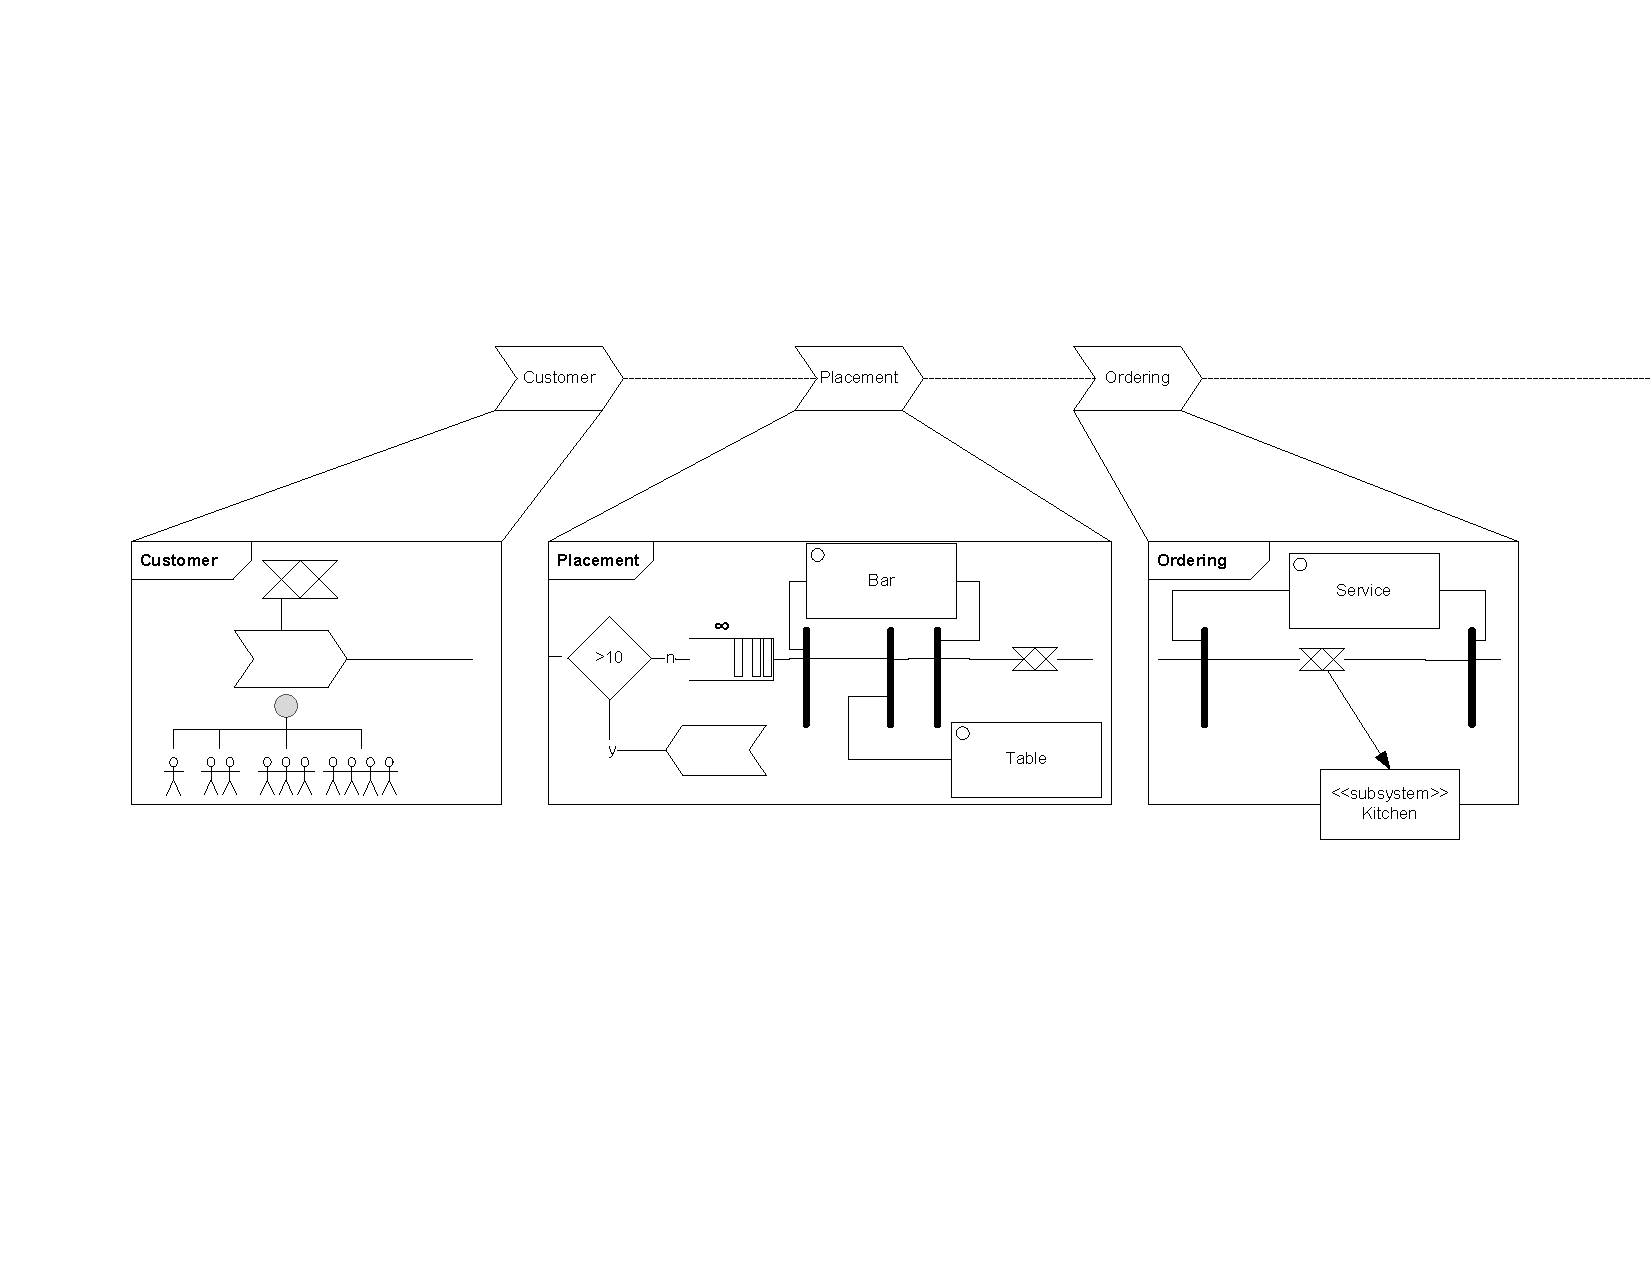
\includegraphics[page=1,trim=2cm 7cm 2cm 5cm, clip=true,width=1.4\textwidth]{../model/Modell_v2.pdf}
				\caption[Hardrock Flow Diagramm Teil1]{Hardrock Flow Diagramm Teil1}
				\label{flowDiagramm1}
		\end{figure}
		
		\subsection{Customer}
		Gäste werdem in Gruppen von eins bis vier Personen erzeugt. Die Erzeugung unterliegt einer definierten Verteilung.
		
		\subsection{Placement}
		Gäste warten in einer beliebig langen Queue, bis eine Platzressource zur Belegung an der Bar frei wird. Die Platzressource wird freigegeben, sobald eine freie Tischressource belegt werden kann.
		
		\subsection{Ordering}
		Während einer Bestellung wird die Bedienung als Ressource belegt und anschliessend wieder freigegeben.
		
		
		\begin{figure}[H]
				\includegraphics[page=2,trim=2cm 7cm 2cm 5cm, clip=true,width=1.4\textwidth]{../model/Modell_v2.pdf}
				\caption[Hardrock Flow Diagramm Teil2]{Hardrock Flow Diagramm Teil2}
				\label{flowDiagramm2}
		\end{figure}
		
		\subsection{Dinnering}
		Gäste warten, bis die Bestellung zubereitet wurde (Verteilfunktion), für die Auslieferung der Teller wird die Ressource Tellerbringer für eine bestimmte Zeit (Verteilfunktion) belegt. Die Dauer des Essens wird ebenfalls mittels einer Verteilfunktion modelliert.
		
		\subsection{Payment}
		Für die Bezahlung ist bis jetzt kein Szenario definiert
		
		\subsection{Exit}
		Gäste geben die belegte Ressource Tisch wieder frei und verlassen das Restaurant.
		\begin{figure}[H]
				\includegraphics[page=3,trim=2cm 12cm 14cm 2cm, clip=true,width=0.5\textwidth]{../model/Modell_v2.pdf}
				\caption[Hardrock Flow Diagramm Kitchen]{Hardrock Flow Diagramm Kitchen}
				\label{flowDiagrammKitchen}
		\end{figure}
		
		\subsection{Kitchen}
		Die Bestellung der Gruppe wird in einzelne Unterbestellungen aufgesplittet und kann parallel verarbeitet werden. Eine Unterbestellung belegt für die Zubereitung einen Koch.
		
\end{landscape}

		\subsection{Entitäten}
		Zusammengefasst sind in der Modellierung des Systems die folgenden Entitäten vorhanden.
		
			\begin{itemize}
		\item Vor der Türe:
			\begin{itemize}
				\item Queue: Ankommende Gäste
			\end{itemize}
		\item Küche
			\begin{itemize}
				\item Agents: Köche
			\end{itemize}
		\item Bedienung
			\begin{itemize}
				\item Agents: Bedienpersonal, Tellerbringer
			\end{itemize}
		\item Bar
			\begin{itemize}
				\item Queue: Anzahl Warteplätze
			\end{itemize}
		\item Tische
			\begin{itemize}
				\item Ressourcen: Anzahl Plätze
			\end{itemize}
	\end{itemize}
	\begin{itemize}
		\item Gäste
		\item Entities: Gruppen von 1-4 Personen 
	\end{itemize}


\chapter{Simulation mit Arena}
	\section{Customer}			
		\subsection{Verteilung der ankommenden Gäste}
			Um die Verteilung des Andrangs, insbesondere die beiden Spitzenzeiten am Mittag und am Abend, zu simulieren, nutzen wir einen Schedule.	
			Die Ankunftsrate im Scheduler ist ??? negativ exponential verteilt.
	
			\begin{figure}[H]
				\centering
					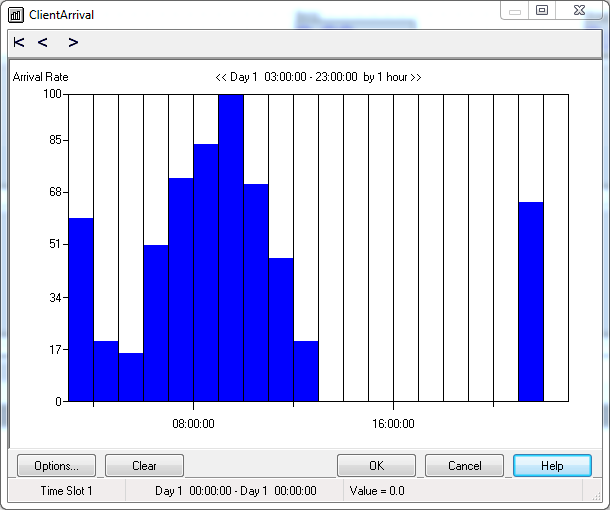
\includegraphics[width=0.75\textwidth]{img/scheduler.png}
					\caption[Arrival Sceduler in Arena]{Ankunfts Sceduler in Arena}
					\label{arrivalSceduler}
			\end{figure}
	
			\subsubsection{Gruppengrösse}
			Einer angekommenen Entität wird anschliessend eine zufällige Gruppengrösse zwischen eins und vier Personen zugeteilt. Dazu wird eine Triangularfunktion mit einem Mittelwert von 2 verwendet und der Ausgabewert auf die nächste ganze Zahl gerundet.
			
	
	\section{Placement}		
		\subsection{Überlauf am Eingang}
			Warten zu viele Gäste vor dem Eingang, werden weitere Gruppen abgeschreckt und kehren wieder um.
		
			Für die Simulation wird eine fixe Grösse verwendet: 			Befinden sich in der EntryQueue weniger als 10 Gruppen, so stellt sich die neue Gruppe an, andernfalls nicht. Mittels einem alternativen Dispose werden die abgeschreckten Gruppen gezählt.
			
			
		\subsection{Assignement und Release von Warteschlange, Bar und Tisch}
			In Arena wird das Assign/Release mittels Ressourcen umgesetzt. Als erstes wird die EntryQueue zugewiesen. Sobald an der Bar Plätze frei werden, wird die BarQueue assigned. Erst wenn der Platz an der BarQueue assigned ist, wird die EntryQueue released. Genau gleich wird für den Wechsel von der Bar an den Tisch verfahren.
	
	
		\subsection{Laufweg der Gäste von der Bar zum Tisch}
			Für den Weg von der Bar zum Tisch wird eine Uniformverteilung von eins bis fünf Minuten eingesetzt. Der Grund liegt darin, dass sich die Gruppen im Restaurant oft weit auseinander setzen. Es entstehen unterschiedliche Laufzeiten, da Tische näher oder weiter entfernt von der Bar platziert sind. Da die Entfernung der Tische keine Häufung aufweist und wir von einer gleichmässigen Auslastung aller Tische ausgehen, wird die Wegverteilung als uniform angenommen.
	
	
	\section{Ordering}			
		\subsection{Bestellvorgang}
			Das Erreichen des Tisches und die Bestellung werden zusammengefasst und mittels einer Triangularverteilung mit einem Mittelwert von 6 sowie einem Minimum von 3 und Maximum von 8 abgebildet. Pro Person am Tisch wird eine Minute aufgeschlagen, um die Abhängigkeit der Bestellzeit von der Gruppengrösse zu realisieren. Zudem ist in dieser grosszügigen Zeitberechnung der Anteil für einen zweiten Besuch am Tisch und die zusätzlichen Aufgaben wie Bereitmachen und Abräumen des Tisches enthalten.
	
	
	\section{Preparation}	
		\subsection{Verteilung der Zubereitungszeit}
			Für die Verteilung der Kochzeit wählen wir eine Normalverteilung mit einem Mittelwert von fünf und einer Standardabweichung von drei Minuten. Da im Hardrock verschiedenste Speisen zubereitet werden, von Salaten über Hauptgängen bis Desserts, ist die Normalverteilung hier die sinnvollste Abbildung. Die Kochzeit wird so kurz gewählt, weil ein guter Koch durch kochen von mehreren Menüs gleichzeitig Synergien nutzen kann.
	
	
		\subsection{Gruppenbestellungen}
			Gruppen bestellen gemeinsam und erhalten ihr Essen zum gleichen Zeitpunkt, gekocht wird es jedoch unabhängig. Um dies abzubilden, verwenden wir da folgende Vorgehen: Die Bestellung der Gruppe wird in der Küche dupliziert und damit werden bis zu vier Unterbestellungen simuliert. Vor dem Ausliefern werden die Unterbestellungen wieder zu einer Gesamtbestellung zusammengefügt.
			
			
	\section{Dinnering}
		\subsection{Bestellungsauslieferung}					
			Die Tellerbringer liefern immer nur Gesamtbestellungen an eine Gruppe aus. Darum wird Bestellung nur ein Tellerbringer benötigt, der bis zu vier Teller (maximale Gruppengrösse) zum Tisch bringt. Zur Simulation wird die Laufzeit von der Theke bis zum Tisch in einer Uniformverteilung von einer halben bis vier Minuten abgebildet.


		\subsection{Essen}
			Das Essen dauert zwischen 15 Minuten und einer Stunde. Einzelne Gänge des Essens werden nicht konkret unterschieden, sondern nur implizit über die Dauer des Aufenthalts am Tisch in einer Verteilfunktion simuliert. Genutzt wird eine Triangularverteilung mit einem Mittelwert von 40 Minuten.\\
			
	\section{Szenarien}
		Zur einfacheren Realisierung der Szenarien werden Controls gesetzt, um die Parameter für jedes Szenario ohne grossen Aufwand variieren zu können.\\
		
		\csvautotabular{szenario.csv}
		
		Die Szenarien sollen in einem ersten Schritt aufzeigen, in welcher Grössenordnung sich die Anzahl der benötigten Servicekräfte, Tellerbringer und Köche zueinander bewegt.
			
		\subsection{Szenarienoptimierung}
		Nach einer ersten Simulation hat sich herausgestellt, dass einige der oben definierten Szenarien gleich von Anfang an ausgeschlossen werden können. So zeigte sich, dass die Anzahl der Tellerbringer und Servicekräfte nicht über der Anzahl Köche liegen kann. Dies wurde ersichtlich, weil sich der Umsatz und damit der Durchsatz (Servicezeiten) im System nicht änderten, wenn die Anzahl der Tellerbringer und Servicekräfte variiert wurden, wenn sie überhalb der Anzahl der Köche lag. Lediglich deren Utilization verringerte sich bei einer Erhöhung der Anzahl.
		 Ebenso konnte ausgeschlossen werden, dass die Anzahl der Köche um einen Faktor von mehr als ca. 4 über der Anzhal der Servicekräfte und des Tellerbringer liegt.  
		
		\subsection{erste Selektion}
			Bezogen auf die Umsatzoptimierung lassen sich aus den besten vier und den schlechtesten vier Szenarien die folgenden Tendenzen ableiten:
			\begin{itemize}
				\item Es werden viele Köche benötigt. 
				\item Tellerbringer braucht es sehr wenige.
				\item Servierpersonal wird etwa halb so viel wie Köche und doppelt so viele wie Tellerbringer benötigt.
			\end{itemize}
		
			Aus diesen Daten entnehmen wir anschliessend den besten Fall (8 Servierpersonal, 4 Tellerbringer und 16 Köche) und analysieren diesen detailierter an:
		
			\begin{itemize}
				\item Der Service ist mit fast 90\% zu hoch ausgelastet. Konkret ist das Personal nicht nur zu den im Scheduler definierten Spitzenzeiten komplett ausgelastet, sondern über den ganzen Zeitraum ausser in den Nachmittagsstunden. 				\item Die Tellerbringer sind zwar über die ganze Simulationszeit regelmässig ausgelastet, insgesammt jedoch zu wenig.
				\item Die Köche sind sehr konstant und über die gesamte Simulationszeit ausgelastet.
			\end{itemize}
			
			
		\subsection{zweite Selektion}
			Als erstes erhöhen wir die Anzahl Simulationsdurchgänge von 10 auf 100, um stabilere und vertrauenswürdigere Resultate zu erhalten.
			
			\subsubsection{Servierpersonal}
				In einer erneuten Simulation wird nur die Anzahl Servierpersonal zwischen 8 und 14 variiert, während die Anzahl Tellerbringer bei 4 und die Anzahl Köche bei 16 bleibt.
				
				Aus der erneuten Simulation geht hervor, dass sich die optimale Anzahl der Servicekräfte um 11 bewegt.
				
			\subsection{Tellerbringer}
				In einem weiteren Schritt fixieren wir das Servierpersonal bei 11 und die Köche bie 16 Personen, variieren aber die Tellerbringer zwischen 2 und 6.
				
				Aus den Ergebnissen der Simulationsläufe geht hervor, dass die optimale Anzahl Tellerbringer bei den schon zuvor gewählten vier liegt.

			\subsection{Köche}
				Im letzen Schritt fixieren wir die Tellerbringer und das Servierpersonal, variieren stattdessen die Köche zwischen 11 und 18 Personen.
				
				Die optimale Anzahl Köche liegt bei 14. Daraus ergibt sich ein Verhältnis von 11:4:14 oder 0.8 Servicekräfte auf 0.3 Tellerbringer auf einen Koch.

		
		\subsection{Dritte Selektion}
			Nach der einzelnen Selektion muss überprüft werden, ob die einzelnen Optimierungen zu globalen Veränderungen geführt haben.
			
			Dazu erstellen wir 27 Szenarien, die das Servicepersonal zwischen 10 und 12, die Tellerbringer zwischen 3 und 5 sowie die Köche zwischen 13 und 15 variieren.
			
			Die vier Besten Resultate dieser Simulation zeigen die Besten bisher gehabten Resultate. Alle Resultate benötigen 10 Servierkräfte, die Tellerbringer variieren zwischen 4 und vier und die Köche zwischen 13 und 15. Der Beste Fall erhalten wir mit 10 Servierkräften, 3 Tellerbringer und 14 Köchen.
			
		
		\subsection{Vierte Selektion}
			Nach der Optimierung des Personals geht es noch um die Optimierung der Bargrösse.
			
			
			
			
	\section{Plausibilitäts-Checks}
	Zur Überprüfung der Plausibilität des aufgebauten Arena Modells experimentierten wir mit verschiedenen Parametern. Dabei sind einige Dinge aufgefallen:
	\begin{itemize}
		\item Die minimale Grösse der Bar muss der grösst möglichen Gruppengrösse (in unserem Fall 4) entsprechen. Andererseits können Gruppen, die grösser als die Bar sind, gar nicht ins Restaurant eintreten.
		Dieses Szenario entspricht nicht ganz der Realität. In der Realität bestehen grosse Gruppen aus kleineren Gruppen. Daher wird ein Teil einer grossen Gruppe bereits das Restaurant betreten, während die Restlichen noch draussen warten.\\
		$\rightarrow$ Da wir eine Bar zwischen 10 und 50 Plätzen anstreben und die Gruppen eine maximale Grösse von vier Personen ausweisen, spielt diese Gegebenheit keine Rolle.
		\item Fünf Angestellte im Service und drei Tellerbringer sind trotz 250 Gästen zu wenig ausgelastet. Das scheint für die Realität wenig plausibel.\\
		$\rightarrow$ Als Korrektur werden die Laufzeiten für das Bedienpersonal und die Tellerbringer angepasst.
		\item Den Flaschenhals in der Simulation stellen die Köche dar. Die tiefe Utilization des Bedienpersonals ergibt sich daraus, dass die Zubereitung der Essen zu lange dauert. Um dieses Verzerrung zu beheben, muss die Anzahl der Köche im Verhältnis zur Anzahl Bedienpersonal erhöht werden.
		
		Gleichzeitig bringt das Servierpersonal in der Realität noch Getränke, Speisekarte, Gedecke, weist dem Gast den Tisch, räumt ab und steht für Fragen zur Verfügung.
		$\rightarrow$ Wir verzichten in unserer Simulation darauf, dies abzubilden. Da die Zeit für die Bedienung aber grosszügig berechnet ist, können die zusätzlichen Zeiten als darin enthalten betrachtet werden.
		\item Die benutzten Zeitvariablen, zur Erfassung von Zeitstempeln im System basieren auf TNOW. Wobei TNOW scheinbar kein Stempel zurückgibt, mit dem gerechnet werden kann.\\
		$\rightarrow$ TNOW muss zuerst in Basetime konvertiert werden. Wobei noch beachtet werden muss, das Basetime vom Run Setup abhängig ist.
	\end{itemize}
			
	\section{Umsatz}
\noindent
	Um den generierten Umsatz zu berechnen, setzen wir die folgenden Werte ein:
Die Kosten für Angestellte sind konstant und nicht von der Anzahl Bestellungen / Besucher abhängig. Deshalb wird wird der Lohn den Ressourcen als Kosten fix zugeteilt.

\begin{tabularx}{\textwidth}{|l|l|X|}
		\hline
		\textbf{Bezeichnung} & \textbf{Preis CHF} & \textbf{Verteilung}  \\
		\hline
		Menu & 20-60 & TRIA(20,30,60)  \\
		\hline
		Stundenlohn Koch & 25 & konstant (Mittelwert)\\
		Stundenlohn Tellerbringer & 20 & konstant (Mittelwert) \\
		Stundenlohn Servicepersonal & 25 & konstant (Mittelwert)\\
		\hline
\end{tabularx}
	
\chapter{Auswertung}
	\section{If Questions}
		\begin{itemize}
			\item \textbf{Was passiert, wenn wir die Anzahl Köche variiert wird?} \\
				Die Köche bringen eine grössere Menge an Bestellungen durch in der gleichen Zeit. Das Servicepersonal ist besser ausgelastet. Sobald das Verhältnis von Köchen zu Servicepersonal 1.4:1 übersteigt, sind die Servierkräfte kommplett ausgelastet, bzw. überlastet. Die Tellerbringer sind überlastet, sobald das Verhältnis von Köchen zu Tellerbringern 4.7:1 übersteigt.
			\item \textbf{Was passiert, wenn die Anzahl Köche verringert wird?} \\
				In der Küche stauen sich die Bestellungen. Die Gäste müssen zu lange auf das Essen warten. Zu wenige neue Gäste können in das Lokal eintreten, das Servierpersonal und die Tellerbringer sind ab den genannten Grenzen nicht mehr ausgelastet.
			\item \textbf{Was passiert, wenn die Anzahl Tellerbringer erhöht wird?}\\
				Sind zu viele Tellerbringer vorhanden, sind diese nicht ausgelastet und stehen herum.
			\item \textbf{Was passiert, wenn die Anzahl Tellerbringer verringert wird?}\\
				Sind weniger Tellerbringer als oben erwähnt vorhanden, stauen sich die gekochten Bestellungen in der Küche. Die Gäste erhalten wiederum die Bestellungen verspätet, belegen das Lokal länger und insgesammt sinkt die Anzahl Bestellungen, die durchgebracht werden können.
			\item \textbf{Was passiert, wenn die Anzahl Servicekräfte erhöht wird?}\\
				Werden die Servicekräfte erhöht, können mehr Bestellungen aufgenommen werden. Sobald das oben genannte Verhältnis zu den Köchen überstiegen wird, Stauen sich die Bestellungen in der Küche, das Servierpersonal ist unterausgelastet.
			\item \textbf{Was passiert, wenn die Anzahl Servierkräfte verringert wird?}\\
				Die Servierkräfte können weniger Bestellungen aufnehmen. Die Küche und die Tellerbringer sind weniger stark ausgelastet.
			\item \textbf{Was passiert, wenn die Anzahl Plätze an der Bar verändert werden?}\\
				Wird die Platzzahl erhöht, so ist die Schlange vor der Türe kleiner und weniger Leute gehen wieder nach Hause. Das Restaurant ist länger besetzt und mehr Umsatz wird generiert. Ist die Bar zu gross, führt der Verzögerungseffekt dazu, dass Gäste noch nach Betriebsschluss im Lokal sind.
				
				Ist die Bar zu klein, gehen viele Leute wieder nach Hause, weil die Schlange vor der Tür zu lang ist. Weniger Gäste durchlaufen das Lokal und weniger Umsatz wird generiert.
			\item \textbf{Was passiert, wenn die Grösse der akzeptablen Schlange variiert wird, bis Gäste wieder nach Hause gehen?}\\
				Wird die Grösse angehoben, gehen weniger Leute nach Hause. Es braucht Mehr Personal im Lokal und die Gäste verbleiben durch den Verzögerungseffekt wie bei der Bar möglicherweise bis nach Betriebsschluss.
				
				Wir die Grösse verkleinert, so gehen mehr Leute nach Hause. Es wird weniger Personal benötigt und weniger Umsatz generiert.
		\end{itemize}


\appendix
\chapter{Präsentation Projektvorstellung}
\begin{center}
	\includegraphics[page=1,angle=180, scale=0.67]{media/presentation-hardrock-slides.pdf}
\end{center}
\begin{center}
	\includegraphics[page=2,angle=180, scale=0.8]{media/presentation-hardrock-slides.pdf}
\end{center}
\begin{center}
	\includegraphics[page=3,angle=180, scale=0.8]{media/presentation-hardrock-slides.pdf}
\end{center}
%\includepdf[pages=1-3,angle=180, scale=0.9]{media/presentation-hardrock-slides.pdf}

\listoffigures

\begin{landscape}
\chapter{Projekt Log}
%git log --no-merges --pretty=format:'%ci: %d %s <%an>' > documentation/gitLog.txt
\verbatiminput{gitLog.txt}
\end{landscape}

\chapter{Materialnachweise}
\section{Titelblatt}
\begin{tabularx}{\textwidth}{|Xlr|}
		\hline
		Logo Hardrock & www.hardrock.com & 25.03.2013 \\
		\hline
\end{tabularx}

\end{document}
